%&tex

\chapter{Experiments and benchmarks}\label{chp:benchmarks}

In this chapter we apply our model on an artificial self-driving dataset, running several
experiments and measuring how good our models perform with each setup. The thinking behind this
benchmarking of models is to provide an initial screening to find the best possible SPN to use on
the real-world testing scenario.

We first describe the different pre-processing transformations applied on the dataset. We then show
results on accuracy for each of the models and pre-processing transformations. Finally we show how
fast each model is, train and test-wise.

\section{Pre-processing}

Before training and inference, we apply different image transformations to the dataset. As
mentioned in~\autoref{chp:modelling}, we use three main transformations: binarization, quantization
and equalization. In all cases we first convert the original RGB colored dataset to grayscale.

\subsection{Binarization}

The binarization process was done by first converting the original dataset to grayscale, followed
by applying a gaussian blur filter with a $(1, 1)$ kernel and $(1, 1)$ standard deviation, and
finally using Otsu's binarization. We chose this particular process since standard hard threshold
binarization was unable to produce clear images of the track lines.

\begin{figure}[h]
  \centering
  
\includegraphics[scale=1.75]{imgs/binary_left_h.png}
  
\includegraphics[scale=1.75]{imgs/binary_up_h.png}
  
\includegraphics[scale=1.75]{imgs/binary_right_h.png}
  \caption{Binarization using hard threshold.\label{fig:bin-hard}}
\end{figure}

\autoref{fig:bin-hard} shows how hard thresholding can produce noisy images, as the applied
threshold does not depend on local neighborhoods. Images are labeled as left, up and right
respectively.

\begin{figure}[h]
  \centering
  
\includegraphics[scale=1.75]{imgs/binary_left.png}
  
\includegraphics[scale=1.75]{imgs/binary_up.png}
  
\includegraphics[scale=1.75]{imgs/binary_right.png}
  \caption{Binarization using Otsu's threshold.\label{fig:bin-otsu}}
\end{figure}

\autoref{fig:bin-otsu} shows a sample of the dataset after applying Otsu's binarization.

\subsection{Quantization}

The Gens-Domingos algorithm, as mentioned in~\autoref{chp:structure}, has two main steps: a
clustering phase and an independency test part. Our independency test implementation in specific
uses the standard G-test statistical independence test based on contingency tables, where each
frequency of the categories of each two variables are laid out on a matrix and their likelihood
ratios are computed. This test takes only $\bigo(n m)$, where $n$ and $m$ are the number of
categories of each variable, but each two variables must be tested pairwise with all others, and
although we use a spanning-tree heuristic, it still grows fast with $n$ and $m$.

We empirically found that $\max\{n,m\}$ and training set size are directly correlated to the
model's accuracy and speed. If $n$ and $m$ are big and the training set size is small, then
accuracy will fall. On the other hand, accuracy increases if $n$ and $m$ are small and the training
set is small. However, when both $n$, $m$ and training set are big, we achieve much better accuracy
results, but inference speed increases as well.

\begin{figure}[h]
  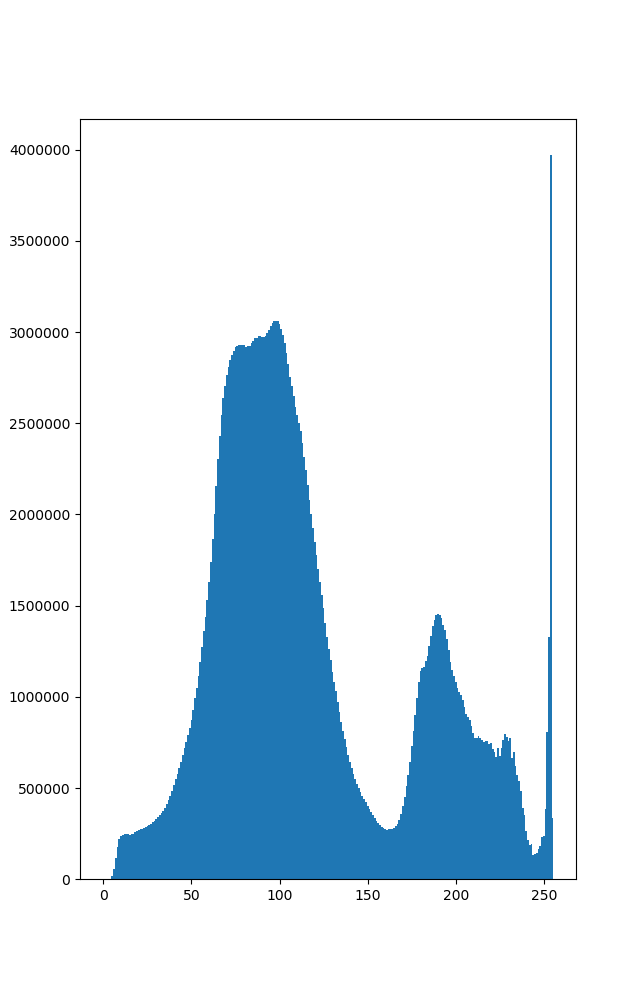
\includegraphics[scale=0.3]{imgs/hist_8.png}
  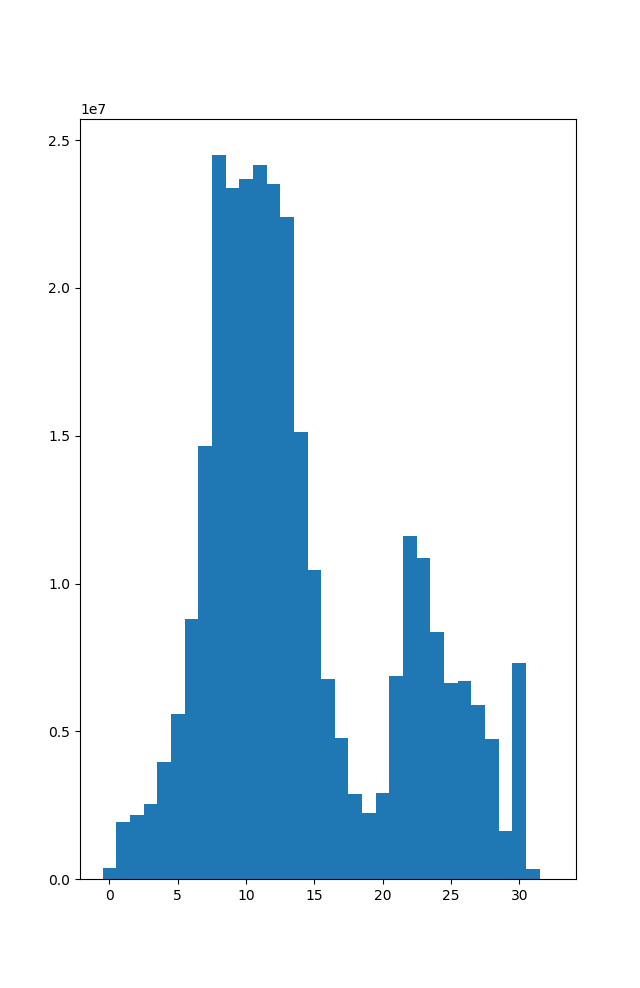
\includegraphics[scale=0.3]{imgs/hist_5.png}
  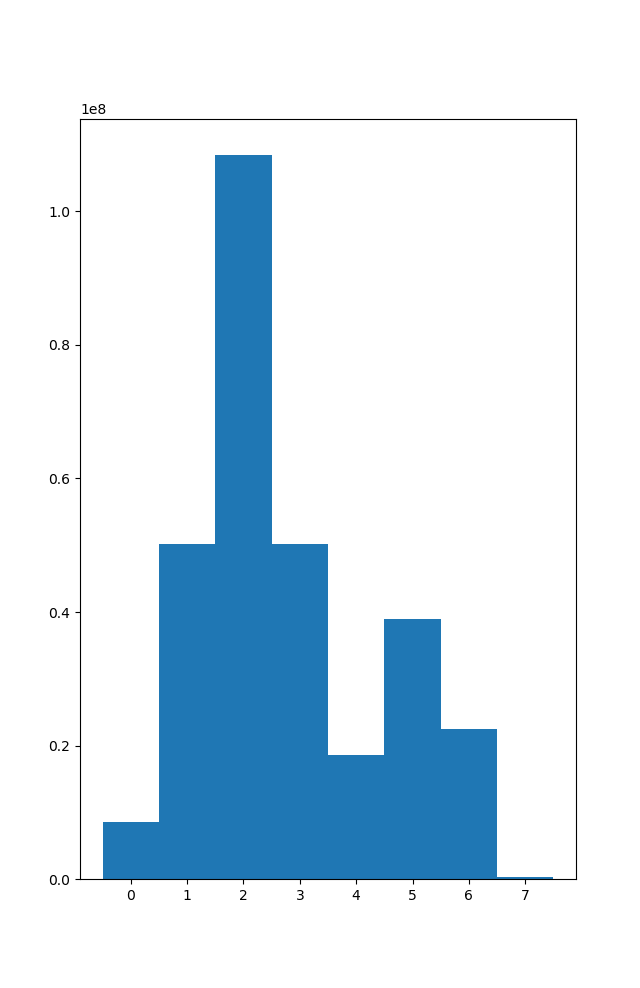
\includegraphics[scale=0.3]{imgs/hist_3.png}
  \caption{Histogram for dataset pixel values on 8-bit, 5-bit and 3-bit image
    resolutions.\label{fig:hist-orig}}
\end{figure}

A possible explanation for poor results with small training sets is the low number of pixel
intensity values for too extreme values, as there are fewer samples where pixels are either too
bright or too dark, as~\autoref{fig:hist-orig} shows.


Quantizing the dataset resulted in a significant improvement in accuracy to the model when training
with a small set of images ($\leq$ 300). We found that when we increased the number of training
images, accuracy depended less on quantization, but inference time increased, as the model grew in
depth. We thus needed to find a balance between network complexity and accuracy.

We faced two possible solutions to this problem. Either implement an exact independence test, such
as the Fisher exact test (\cite{fisher-exact}), or perform equalization on the dataset. The former
was unfortunately not an option, as we found that there were no libraries in Go or C that provided
a general case implementation of the Fisher exact test, and implementing our own within our time
constraints was out of question. We chose the latter, applying histogram equalization on the entire
dataset.

\subsection{Equalization}

Equalization was done using OpenCV. We attempted two methods of histogram equalization: traditional
equalization through brightness and contrast normalization, and Contrast Limited Adaptive Histogram
Equalization (CLAHE) (\cite{clahe}). We found that the CLAHE method resulted in images that were
very similar to the output of the traditional method. Since these transformations are also expected
to be applied on-the-fly during inference, we chose the standard equalization for its speed.
\autoref{fig:hist-eq} shows how the dataset pixel histogram looks like after equalization.

\begin{figure}[h]
  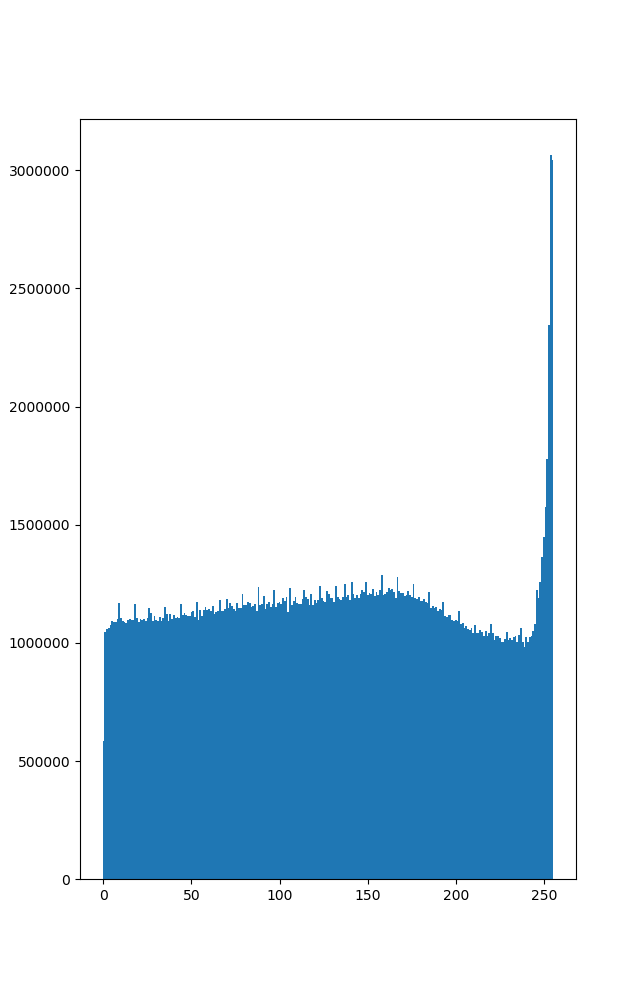
\includegraphics[scale=0.3]{imgs/hist_8_eq.png}
  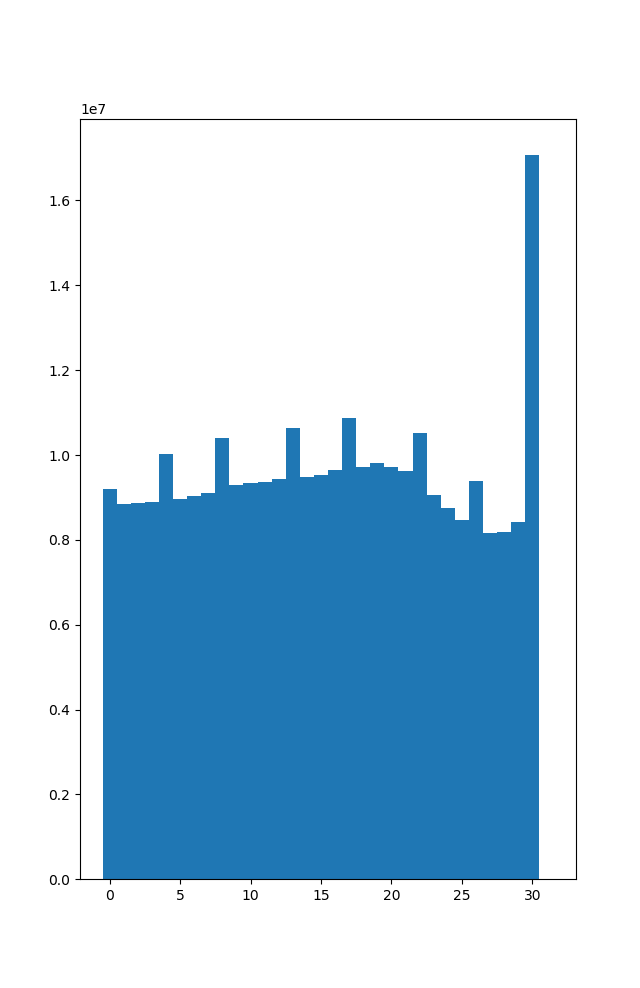
\includegraphics[scale=0.3]{imgs/hist_5_eq.png}
  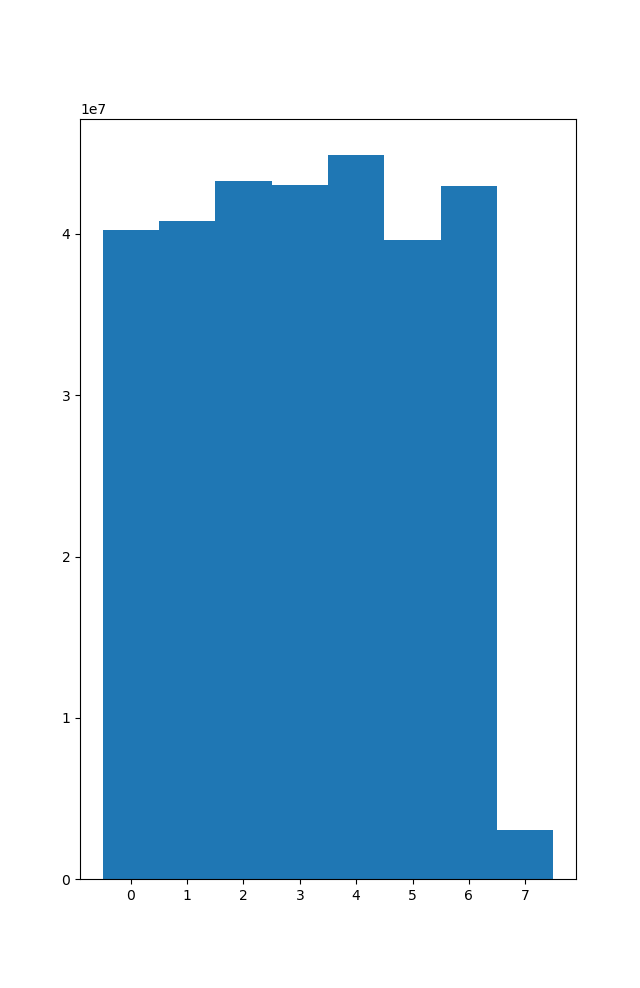
\includegraphics[scale=0.3]{imgs/hist_3_eq.png}
  \caption{Histogram for equalized dataset with 8-bit, 5-bit and 3-bit image
  resolutions.\label{fig:hist-eq}}
\end{figure}

When coupling quantization and equalization, we were able to achieve $\approx$81\% accuracy.
Interestingly, these transformations proved to be harmful for the Dennis-Ventura architecture. In
fact, the structure yielded better results with higher resolutions compared to lower. Equalization
also had little to no effect on this architecture, increasing accuracy in 1\% or 2\% when training
with a small dataset, and having no effect when training with many samples. We attribute this
phenomenom to the classification architecture we discussed in~\autoref{chp:structure}. Since each
sub-SPN is essentially modelling each class as a separate, independent image model to the other
classes, the more details in the image, the easier the model can distinguish from other label
images.  Furthermore, since the Dennis-Ventura algorithm does not need to run an independence test,
it does not suffer from its drawbacks and thus does not depend on an equalized histogram.

\section{Setups}

For our experiments, we tested two structure learning algorithms, the Dennis-Ventura and
Gens-Domingos architectures, and for each of these models we evaluated accuracy when applying
either generative or discriminative weight learning. We additionally ran tests without applying
weight learning to serve as reference.

For the Dennis-Ventura algorithm, we discarded pre-clustering, opting to use the classification
architecture mentioned in~\autoref{chp:structure}, as it resulted in much better accuracy. We also
fixed the number of sums per region and gaussians per pixel to four, and the similarity threshold
to $0.975$.

For the Gens-Domingos algorithm, we tested two implementations. The first uses $k$-means for the
clustering step with $k=2$. The second uses DBSCAN, with parameters $\epsilon=4$ the maximum radius
of a point neighborhood, and $m=4$ the minimum number of points to describe a dense region. Both
were set with a $p$-value of $0.01$ for the independence step. We refer to the $k$-means
implementation as $k$-GD, and the DBSCAN variation as DBSCAN-GD.

We found that when using DBSCAN-GD, the resulting structure was too complex, causing inference to
take too long. For instance, when running inference on $k$-GD, average prediction took about $0.4$
second.  When using DBSCAN, the average time of prediction was $12.33$ seconds.  Size-wise, the
DBSCAN variation had a structure 18 times bigger. However, in terms of accuracy, DBSCAN-GD showed
impressive results, with accuracies ranging from 98\% to 100\%. Despite these results, a model that
takes too long for inference is not adequate for a self-driving application. For this reason, we
show only comparisons with the $k$-GD model.

In both training and testing, we first apply image transformations (e.g. quantizing, binarization
or equalization) to the dataset and then train or perform prediction with a particular model. The
applied image transformation is always identical in training and testing. For example, a valid
training pipeline would be choosing to apply 3-bit quantization and equalization to a training
dataset, train an SPN structure using $k$-GD, perform discriminative gradient descent on the
resulting structure to learn its weights, and finally save the model for testing. The equivalent
testing pipeline for this training pipeline would be applying the same image transformation, in our
case 3-bit quantization and equalization, and for each image find the $\argmax_{y\in Y} P(Y=y|X)$.

Both Gens-Domingos and Dennis-Ventura algorithms generate a structure as deep as the number of
training samples. The deeper the structure, the more expressive it is. We found that accuracy with
models trained with 1000 samples had much better accuracies than with 500. However, a more complex
network means inference will take longer. We attempted to keep inference at less than a second per
prediction. This was done by restricting the training dataset to 500 images.

We use a particular set of notations for our experiments. For image transformations, we denote by
$Q_n$ as applying an $n$-bit quantization of the dataset. An $E$ means the dataset was equalized,
and a $B$ means it was binarized. Any combination of image transformation is signalled with a $+$
sign. A $\emptyset$ means there were no image transformations done to the dataset apart from
grayscale conversion.

For learning algorithms, a GD means we are using $k$-means Gens-Domingos and DV Dennis-Ventura.
This is then followed by the weight learning algorithm used. The letters g, d and s mean we either
applied generative gradient descent, discriminative gradient descent or no weight learning.

\section{Accuracy}

In this section we show accuracy results in each setup. All values are in percentage of hits.

\begin{table}[h]
  \centering
  \begin{tabular}{l|c|c|c|c|c|c}
    \hline
    \multicolumn{1}{c}{\bfseries Accuracy (\%)} & \multicolumn{1}{c}{\bfseries DV+g} &
    \multicolumn{1}{c}{\bfseries DV+d} & \multicolumn{1}{c}{\bfseries DV+s} &
    \multicolumn{1}{c}{\bfseries GD+g} & \multicolumn{1}{c}{\bfseries GD+d} &
    \multicolumn{1}{c}{\bfseries GD+s}\\
    \hline
    $B$         & 76.0 & 76.6 & 76.6 & 80.2 & 76.6 & 78.8\\
    $Q_2$       & 75.6 & 76.6 & 76.6 & 78.2 & 80.0 & 77.6\\
    $Q_2+E$     & 75.8 & 76.6 & 76.6 & 79.4 & 78.6 & 78.0\\
    $Q_3$       & 76.0 & 76.6 & 76.6 & 79.6 & 80.6 & 79.2\\
    $Q_3+E$     & 75.2 & 76.6 & 76.6 & 80.2 & 80.2 & 80.2\\
    $Q_4$       & 75.8 & 76.6 & 76.6 & 78.2 & 79.6 & 79.8\\
    $Q_4+E$     & 75.6 & 76.6 & 76.6 & 78.4 & 78.4 & 82.0\\
    $Q_5$       & 76.0 & 76.6 & 76.6 & 80.0 & 78.4 & 78.0\\
    $Q_5+E$     & 75.6 & 76.6 & 76.6 & 79.8 & 81.2 & 78.8\\
    $Q_6$       & 76.0 & 76.6 & 76.6 & 78.8 & 80.6 & 80.8\\
    $Q_6+E$     & 75.6 & 76.6 & 76.6 & 79.2 & 80.6 & 77.6\\
    $Q_7$       & 76.6 & 76.6 & 76.6 & 77.4 & 77.4 & 79.2\\
    $Q_7+E$     & 76.6 & 76.6 & 76.6 & 80.6 & 81.0 & 79.6\\
    $\emptyset$ & 75.6 & 76.6 & 76.6 & 77.6 & 81.6 & 80.4\\
    $E$         & 75.6 & 76.6 & 76.6 & 78.2 & 80.6 & 79.0\\
  \end{tabular}
  \caption{Accuracy values for each possible model permutation.\label{tab:accuracy}}
\end{table}

\autoref{tab:accuracy} shows some interesting results. The first is that generative gradient
descent on the Dennis-Ventura architecture had a small to no negative impact on the performance of
the network.

The Gens-Domingos architecture, on the other hand, achieved better results, but showed a more
unpredictable behavior.

\section{Speed}

\begin{table}[h]
  \centering
  \begin{tabular}{l|c|c|c|c|c|c}
    \hline
    \multicolumn{1}{c}{\bfseries Training (mins)} & \multicolumn{1}{c}{\bfseries DV+g} &
    \multicolumn{1}{c}{\bfseries DV+d} & \multicolumn{1}{c}{\bfseries DV+s} &
    \multicolumn{1}{c}{\bfseries GD+g} & \multicolumn{1}{c}{\bfseries GD+d} &
    \multicolumn{1}{c}{\bfseries GD+s}\\
    \hline
    $B$         & 54m54s & 48m42s & 00m19s & 76m32s & 115m07s& 05m50s\\
    $Q_2$       & 53m46s & 49m09s & 00m17s & 75m51s & 109m49s& 04m44s\\
    $Q_2+E$     & 53m00s & 46m00s & 00m15s & 85m03s & 112m05s& 04m55s\\
    $Q_3$       & 60m19s & 46m36s & 00m15s & 83m34s & 108m23s& 05m23s\\
    $Q_3+E$     & 62m06s & 45m14s & 00m22s & 75m39s & 111m03s& 04m28s\\
    $Q_4$       & 50m14s & 42m58s & 00m18s & 83m00s & 74m25s & 04m39s\\
    $Q_4+E$     & 50m19s & 40m52s & 00m16s & 77m23s & 60m25s & 05m43s\\
    $Q_5$       & 54m22s & 40m41s & 00m15s & 48m57s & 55m39s & 04m55s\\
    $Q_5+E$     & 50m32s & 44m44s & 00m24s & 48m21s & 50m59s & 04m06s\\
    $Q_6$       & 50m54s & 40m36  & 00m14s & 43m59s & 59m38s & 04m19s\\
    $Q_6+E$     & 56m32s & 40m27s & 00m15s & 44m21s & 46m09s & 05m23s\\
    $Q_7$       & 56m58s & 40m16s & 00m15s & 40m46s & 67m04s & 05m52s\\
    $Q_7+E$     & 60m13s & 40m43s & 00m15s & 45m16s & 62m33s & 05m52s\\
    $\emptyset$ & 62m14s & 41m07s & 00m15s & 39m45s & 67m04s & 06m45s\\
    $E$         & 57m23s & 40m35s & 00m15s & 51m37s & 62m33s & 04m58s\\
  \end{tabular}
  \caption{Average time in minutes for training each model.\label{tab:time-training}}
\end{table}

\begin{table}[h]
  \centering
  \begin{tabular}{l|c|c|c|c|c|c}
    \hline
    \multicolumn{1}{c}{\bfseries Inference (secs)} & \multicolumn{1}{c}{\bfseries DV+g} &
    \multicolumn{1}{c}{\bfseries DV+d} & \multicolumn{1}{c}{\bfseries DV+s} &
    \multicolumn{1}{c}{\bfseries GD+g} & \multicolumn{1}{c}{\bfseries GD+d} &
    \multicolumn{1}{c}{\bfseries GD+s}\\
    \hline
    $B$         & 0.58 & 0.64 & 0.79 & 0.44 & 0.48 & 0.47 \\
    $Q_2$       & 0.56 & 0.65 & 0.63 & 0.43 & 0.45 & 0.42 \\
    $Q_2+E$     & 0.62 & 0.63 & 0.61 & 0.49 & 0.45 & 0.33 \\
    $Q_3$       & 0.65 & 0.58 & 0.59 & 0.50 & 0.43 & 0.40 \\
    $Q_3+E$     & 0.57 & 0.56 & 0.69 & 0.42 & 0.45 & 0.34 \\
    $Q_4$       & 0.56 & 0.57 & 0.65 & 0.58 & 0.67 & 0.31 \\
    $Q_4+E$     & 0.57 & 0.55 & 0.61 & 0.60 & 0.62 & 0.37 \\
    $Q_5$       & 0.56 & 0.61 & 0.66 & 0.51 & 0.43 & 0.34 \\
    $Q_5+E$     & 0.57 & 0.56 & 0.62 & 0.48 & 0.39 & 0.33 \\
    $Q_6$       & 0.65 & 0.56 & 0.62 & 0.63 & 0.55 & 0.37 \\
    $Q_6+E$     & 0.57 & 0.56 & 0.60 & 0.65 & 0.35 & 0.34 \\
    $Q_7$       & 0.56 & 0.56 & 0.59 & 0.44 & 0.53 & 0.40 \\
    $Q_7+E$     & 0.56 & 0.56 & 0.58 & 0.46 & 0.58 & 0.42 \\
    $\emptyset$ & 0.64 & 0.56 & 0.58 & 0.42 & 0.74 & 0.52 \\
    $E$         & 0.62 & 0.55 & 0.59 & 0.58 & 0.42 & 0.37 \\
  \end{tabular}
  \caption{Average time in seconds to predict a single image.\label{tab:time-inference}}
\end{table}
